\bookchapter{Power and Safety}\label{ch:hw8}

\section*{Explanation}
A battery stores as much energy as a small bomb for its weight, and a humanoid robot weighs tens of kilograms and falls over. This chapter treats power (batteries, regulators, wires and fuses) and safety (the emergency stop, the safety chain, safe behaviour on failure and the rules of the lab) together, because in a robot they are the same subject: \emph{where does the energy go, and what happens when something breaks?} The rules at the end of the chapter are not optional. Follow them, also when you are in a hurry, especially before a competition.

\section*{Battery basics}
A cell stores charge in ampere-hours (Ah) at a voltage that depends on the chemistry; the energy is $E=U\cdot Q$ in watt-hours (Wh). Common chemistries (per cell, typical values):
\begin{center}
\renewcommand{\arraystretch}{1.25}
\begin{tabular}{p{3.0cm}p{2.9cm}p{6.8cm}}
\textbf{Chemistry} & \textbf{Voltage (empty--nominal--full)} & \textbf{Remarks}\\ \hline
LiPo (pouch) & $3.0$--$3.7$--$4.2$\,V & high current, light, soft pouch that swells when damaged; the classical drone/RC battery; the most sensitive to abuse\\
Li-ion (cylindrical, e.g.\ 18650, 21700) & $3.0$--$3.6$--$4.2$\,V & more energy per kg, metal can, less aggressive, standard for e-bikes and many robots\\
LiFePO$_4$ (LFP) & $2.5$--$3.2$--$3.65$\,V & very safe and long-lived (thousands of cycles), heavier\\
NiMH & $1.0$--$1.2$--$1.4$\,V & robust and harmless, low energy density; AA cells\\
\end{tabular}
\end{center}
\subsection*{Series, parallel and the notation \texttt{nSmP}}
Cells in \textbf{series} add the voltage; in \textbf{parallel} they add the capacity (and the current capability). A pack described as \textbf{6S1P} has six cells in series (nominal $6\cdot3.7=22.2$\,V, full $6\cdot4.2=25.2$\,V, empty $6\cdot3.0=18$\,V); \textbf{6S2P} has two such strings in parallel, with twice the capacity.
\begin{center}
\begin{circuitikz}[scale=0.85,transform shape]
  \draw (0,0) to[battery1,l_=$3.7$ V] (0,1.6) to[battery1,l_=$3.7$ V] (0,3.2) to[battery1,l_=$3.7$ V] (0,4.8);
  \draw (0,0) -- (1,0); \draw (0,4.8) -- (1,4.8);
  \node[right,font=\footnotesize] at (1.1,4.8) {$+\ 11.1$ V};
  \node[right,font=\footnotesize] at (1.1,0) {$-$};
  \begin{scope}[xshift=6cm]
  \draw (0,0) to[battery1,l_=$3.7$ V] (0,2) ;
  \draw (1.6,0) to[battery1,l_=$3.7$ V] (1.6,2);
  \draw (3.2,0) to[battery1,l_=$3.7$ V] (3.2,2);
  \draw (0,0)--(3.2,0); \draw (0,2)--(3.2,2);
  \draw (1.6,2)--(1.6,2.6) node[above,font=\footnotesize]{$+\ 3.7$ V};
  \end{scope}
  \node[font=\footnotesize] at (0.5,-0.7) {3S1P: series};
  \node[font=\footnotesize] at (7.6,-0.7) {1S3P: parallel};
\end{circuitikz}
\captionof{figure}{Series cells add voltage, parallel cells add capacity.}
\end{center}
\subsection*{Capacity, C-rate and runtime}
The \textbf{C-rate} expresses a current relative to the capacity: $1$\,C of a $5$\,Ah pack is $5$\,A, $2$\,C is $10$\,A. Cells specify a maximum \emph{continuous} discharge (e.g.\ $20$\,C for a LiPo, only $1$--$3$\,C for many energy-optimised Li-ion cells) and a lower charge rate (typically $\le1$\,C). \textbf{Runtime} follows from the energy and the power drawn:
\[
t=\frac{E_\text{usable}}{P},\qquad E_\text{usable}\approx0.8\,E\ \text{(never use a Li-ion pack down to empty).}
\]
\begin{example}
\textbf{How long does the robot run?} A 6S pack with $5$\,Ah: $E=22.2\cdot5=111$\,Wh. Usable $\approx0.8\cdot111=88.8$\,Wh. The robot draws on average $150$\,W (standing: much of it as copper loss in the joints, Chapter~\ref{ch:hw6}): $t=88.8/150=0.59$\,h $=35.5$\,min. The average current is $150/22.2=6.8$\,A, i.e.\ $1.35$\,C, well within the limits; the peak current, e.g.\ when the robot gets up from the floor ($600$\,W), is $27$\,A, $5.4$\,C: check the continuous and peak ratings of cells \emph{and} the connector, the wires and the BMS.
\end{example}
The voltage of a cell is not constant: it drops while discharging and sags under load because of the internal resistance $R_i$ ($U=U_\text{oc}-R_iI$). The sag is the reason why a robot can switch off in the middle of a step: a short current peak pushes the voltage below the threshold of the electronics.
\begin{center}
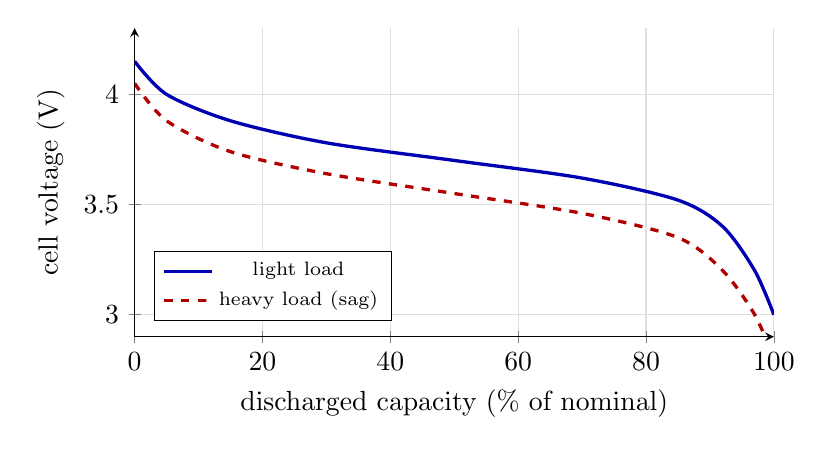
\begin{tikzpicture}
\begin{axis}[width=0.8\textwidth,height=5.5cm,xlabel={discharged capacity (\% of nominal)},ylabel={cell voltage (V)},xmin=0,xmax=100,ymin=2.9,ymax=4.3,grid=both,grid style={gray!25},axis lines=left,legend style={font=\scriptsize,at={(0.03,0.05)},anchor=south west},xlabel near ticks,ylabel near ticks]
 \addplot[blue!70!black,very thick,smooth] coordinates {(0,4.15)(5,4.0)(15,3.88)(30,3.78)(50,3.70)(70,3.62)(85,3.52)(92,3.40)(97,3.2)(100,3.0)};
 \addplot[red!70!black,very thick,dashed,smooth] coordinates {(0,4.05)(5,3.88)(15,3.74)(30,3.64)(50,3.55)(70,3.46)(85,3.35)(92,3.2)(97,3.0)(100,2.8)};
 \legend{light load,heavy load (sag)}
\end{axis}
\end{tikzpicture}
\captionof{figure}{A \emph{schematic} discharge curve of a Li-ion cell (typical shape, not data of a particular cell): flat in the middle, steep at the end, and lower under heavy load.}\label{fig:hw8_dis}
\end{center}

\section*{The battery management system (BMS)}
A pack of several cells must never be treated as one big cell. The \textbf{BMS} watches every cell and: stops charging above $4.2$\,V per cell, stops discharging below the lower limit, limits the current, protects against short circuits, switches off at excessive temperature, and \textbf{balances} the cells so that they stay at the same voltage. Cells are damaged by overcharge (heat, gas, fire), deep discharge (copper dissolves, internal shorts later) and charging when frozen. Rules:
\begin{itemize}[nosep]
\item Use a \textbf{charger made for the chemistry and the cell count}, with balancing, and charge on a non-flammable surface with someone present; never charge overnight unattended.
\item Do not use a swollen, dented or hot pack; do not pierce, short or crush a cell. Damaged packs go into a metal box (or a bucket of sand) and to proper battery collection, never into household waste.
\item For storage of more than a few days: about $50$\,\% charge ($\approx3.8$\,V per Li-ion cell), cool and dry, in a fire-safe bag or box.
\item A Li-ion fire cannot be put out by turning the supply off, since the cell contains its own oxidant; it must be cooled with a lot of water (or isolated and left to burn out) and the room evacuated. The lab needs a defined procedure, and everybody must know where it is written.
\end{itemize}

\section*{Power distribution: the power tree}
The battery voltage is rarely right for all loads: motors take $24$\,V or the battery directly, the computer $12$ or $19$\,V, microcontrollers and sensors $5$ or $3.3$\,V. A \textbf{power tree} lists every rail with its voltage, maximum current, source and protection (draw it for your robot, Figure~\ref{fig:hw8_tree}).
\begin{center}
\begin{tikzpicture}[blk/.style={draw,thick,rounded corners=2pt,minimum width=2.4cm,minimum height=0.8cm,align=center,font=\footnotesize},>={Stealth[length=2.5mm]}]
 \node[blk,fill=red!10] (bat) at (0,0) {Battery\\ 6S, 22.2\,V};
 \node[blk,fill=orange!15] (fuse) at (3.2,0) {Fuse +\\ main switch};
 \node[blk,fill=gray!15] (bms) at (6.4,0) {BMS /\\ contactor};
 \draw[->,thick] (bat)--(fuse); \draw[->,thick] (fuse)--(bms);
 \node[blk,fill=blue!10] (mot) at (3.2,-2.2) {motor drivers\\ (joints) 22\,V};
 \node[blk,fill=green!10] (buck) at (6.4,-2.2) {buck converter\\ 22\,V$\to$12\,V};
 \node[blk,fill=green!10] (pc) at (9.6,-2.2) {onboard PC\\ 12\,V};
 \node[blk,fill=green!10] (b5) at (9.6,-3.8) {buck 5\,V:\\ sensors, MCU};
 \draw[->,thick] (bms.south) -- ++(0,-0.6) -| (mot.north);
 \draw[->,thick] (bms.south) -- ++(0,-0.6) -| (buck.north);
 \draw[->,thick] (buck)--(pc);
 \draw[->,thick] (buck.south) -- ++(0,-1.6) -- (b5.west);
\end{tikzpicture}
\captionof{figure}{A typical power tree. The computer's supply should be separate (and filtered) from the motors, so that motor peaks do not reset the computer.}\label{fig:hw8_tree}
\end{center}

\subsection*{Voltage regulators}
\begin{itemize}[nosep]
\item \textbf{Linear regulator (LDO)}: simple, quiet, but the input current equals the output current, so it burns $(U_\text{in}-U_\text{out})\,I$ as heat.
\item \textbf{Switching (buck) converter}: chops the voltage with a MOSFET (PWM, Chapter~\ref{ch:hw3}) and smooths with a coil and a capacitor; efficiency $85$--$95\,\%$, but electrical noise at the switching frequency.
\end{itemize}
\begin{example}
\textbf{$24$\,V to $5$\,V at $3$\,A.} The output power is $15$\,W. \emph{LDO}: the input current is $3$\,A, $P_\text{in}=24\cdot3=72$\,W, the loss is $(24-5)\cdot3=57$\,W and the efficiency $15/72=21\,\%$: impossible without a huge heat sink. \emph{Buck with $\eta=0.9$}: $P_\text{in}=15/0.9=16.7$\,W, $I_\text{in}=0.69$\,A, the loss $1.7$\,W. Use an LDO only for small currents or for a small dropout, after a buck, e.g.\ for a clean $3.3$\,V for an analogue sensor.
\end{example}

\subsection*{Wires, connectors and fuses}
A wire has resistance $R=\rho L/A$ with $\rho=1.72\cdot10^{-8}\,\Omega$\,m for copper; the loss $RI^2$ heats it, and the voltage drop $RI$ appears at the load.
\begin{example}
\textbf{Wire for a $20$\,A rail.} One metre each way ($L=2$\,m) with $A=1.5$\,mm$^2$: $R=1.72\cdot10^{-8}\cdot2/(1.5\cdot10^{-6})=0.023\,\Omega$; voltage drop at $20$\,A: $0.46$\,V; loss $9.2$\,W in the wire! With $A=4$\,mm$^2$: $R=8.6$\,m$\Omega$, drop $0.17$\,V, loss $3.4$\,W. Thick, short wires for high currents; the twisted pair for signals.
\end{example}
A \textbf{fuse} (or circuit breaker) protects the \emph{wire}, not the device: it must blow before the wire gets hot, so choose its rating \emph{below} the wire's safe current and above the normal peak, and make sure it can interrupt the available short-circuit current of the battery (a LiPo can deliver hundreds of amperes). Put the fuse directly at the battery, in the positive line, before any other part. Connectors must be rated for the current, polarised so that they cannot be reversed (a battery connected the wrong way round kills electronics instantly), and locked against vibration. Add a \textbf{precharge} resistor or a switch for large capacitances (motor drivers), otherwise the connecting spark welds contacts.

\section*{Safety of a robot}
\subsection*{The emergency stop and the safety chain}
An \textbf{emergency stop (E-stop)} is a red mushroom button that removes the power from the actuators \emph{by hardware}, independent of any software. It must be easy to reach (a remote one in your hand when the robot walks), and work when the computer has crashed. Typical design: a \textbf{safety chain}, a series loop of normally closed contacts (E-stop buttons, lid switches, driver fault outputs) that holds a contactor or an enable line. \emph{Any} break in the chain, a pressed button, a cut wire, a lost radio link, opens it: the principle is \textbf{fail-safe}, i.e.\ the safe state is the one that results when energy or signals are \emph{missing}.
\begin{keyidea}[Rules of a safe robot]
(1) A hardware E-stop that cuts the \emph{motor power}; the logic stays on so that you can read the cause. (2) Fail-safe: loss of power, signal or communication leads to the safe state. (3) A \textbf{watchdog} (Chapter~\ref{ch:py12}): the driver must switch off or go limp if the commands are not refreshed within, say, $50$\,ms. (4) Limits on torque, speed, position and temperature \emph{in the driver} and not only in your code. (5) Test the E-stop at every start of the day. (6) Never rely on one single protection.
\end{keyidea}
\subsection*{What is the safe state of a humanoid?}
For a stationary machine the safe state is usually ``motors off''. For a humanoid this is not obvious: if the power is cut while it stands, it falls like a tree, with its whole mass, onto the floor and perhaps onto a person or a hand. Typical solutions are a \textbf{damped stop} (the joints become compliant, with low $K_p$ and some $K_d$, so the robot sinks down), a gantry or a \textbf{safety harness} on a hoist during tests, and the rule that nobody stands within the fall range of the robot during experiments. The energy matters: a $20$\,kg robot at the height of $0.5$\,m has $mgh=20\cdot9.81\cdot0.5=98$\,J of potential energy; its joints can pinch fingers with several hundred newtons.

\subsection*{Hazards at a glance}
\begin{center}
\renewcommand{\arraystretch}{1.25}
\begin{tabular}{p{3.2cm}p{9.5cm}}
\textbf{Hazard} & \textbf{Countermeasure}\\ \hline
Falling robot & harness or hoist for tests, clear zone, soft floor, stop button in hand\\
Pinch and crush points & keep hands away from joints and gears, switch off power for work on the robot, covers\\
Battery fire & BMS, correct charger, fire-safe bag, never unattended, fire extinguisher or sand at hand\\
Short circuit & fuse at the battery, insulate, tools with insulated handles, remove metal jewellery\\
Hot parts & motors and drivers can reach $>80\,^\circ$C; thermal monitoring, wait before touching\\
ESD (electrostatic discharge) & touch ground before handling boards, work on an antistatic mat; ESD can silently damage chips\\
Soldering & $350\,^\circ$C iron in its holder, ventilation (flux fumes), wash hands (leaded solder)\\
Loose wires and cables & strain relief and routing away from moving joints; a cable in a gear is a short circuit later\\
Wireless link lost & a failsafe stop after a timeout, not ``continue last command''\\
\end{tabular}
\end{center}

\subsection*{Procedures for the lab}
\begin{enumerate}[nosep]
\item \textbf{Before power-on:} look at the robot (loose parts, cables, battery fixed), clear the zone, check the E-stop, announce loudly: ``powering on''.
\item \textbf{First test of new software}: robot on the stand or in the harness, feet off the ground, low gains, low torque limits, one hand on the E-stop. Only then on the floor.
\item \textbf{Roles}: one person runs the robot, one is the \emph{spotter} who watches the robot and holds the stop; the spotter has the right to stop any test at any time without explanation.
\item \textbf{Work on the robot only when it is powered off} and the battery is disconnected; tag and lock the battery out.
\item \textbf{After the test}: switch off, disconnect the battery, charge or store it correctly, write down what happened (a log helps the next student).
\end{enumerate}
\begin{aibox}[Safety and learned policies]
A neural-network policy is a function that was trained on a simulation and can output surprising actions in situations it has never seen. Therefore the safety layer must \emph{not} be part of the network: clipping of torques and speeds, joint limits, a fall detector (IMU tilt $>$ threshold, Chapter~\ref{ch:hw4}) that triggers the damped stop, and the watchdog run as simple, verified code outside the policy, and in the driver hardware wherever possible.
\end{aibox}

\section*{Practice problems}
\begin{enumerate}[label=\textbf{\thechapter.\arabic*}]
  \item A pack is 4S3P with cells of $3.6$\,V nominal and $3$\,Ah. Compute nominal voltage, capacity, energy and the maximum voltage when fully charged ($4.2$\,V per cell).
  \item A 6S pack with $8$\,Ah is used at $25$\,A. Calculate the C-rate, the power at nominal voltage ($3.7$\,V per cell) and the runtime to $80\,\%$ discharge.
  \item The internal resistance of the pack in problem 2 is $60$\,m$\Omega$. Compute the voltage sag and the loss in the battery at $25$\,A, and the voltage at the load if the open-circuit voltage is $23$\,V.
  \item A buck converter ($\eta=0.92$) supplies $12$\,V at $5$\,A from $24$\,V. Compute the input power and current and the loss. Compare with a linear regulator.
  \item A $2$\,m cable (round trip) of $2.5$\,mm$^2$ copper carries $30$\,A. Compute resistance, voltage drop and heat loss.
  \item Give two reasons why a fuse is placed directly at the battery, in the positive line.
  \item Why is a normally \emph{closed} loop better for the E-stop than a normally \emph{open} switch that is closed when the button is pressed? Explain ``fail-safe'' with this example.
  \item A watchdog timeout of $50$\,ms and a robot speed of $1$\,m/s (a falling arm tip, say). How far can the part travel after the last valid command before the driver reacts? Is it acceptable at $200$\,ms?
  \item Compute the potential energy of a $20$\,kg robot at $0.5$\,m and at $1.0$\,m. Compare to the energy of a $0.5$\,kg ball thrown at $10$\,m/s.
  \item[\textbf{\thechapter.10}$\star$] Draw (by hand or TikZ) the power tree for a robot with a 6S battery, $22$\,V motor drivers (peak $40$\,A), a $12$\,V onboard PC ($60$\,W) and $5$\,V sensors ($10$\,W); choose fuse ratings, and compute the buck converter input currents (efficiency $0.9$) at $22.2$\,V. Add the E-stop to the drawing and say what it switches.
\end{enumerate}
